\newpage

\section{Задание 1.}

Записать как двойной интеграл, сделать рисунок области и поменять порядок
интегрирования.
$$\int_{0}^{1}\, dy \int_{0}^{\sqrt{y}} f \, dx  + \int_{1}^{\sqrt{2}} \, dy\int_{0}^{\sqrt{2-y^2}} f \, dx $$

Чтобы записать как двойной интеграл, нужно определить область, по которой происходит интегрирование. Можно заметить, что по оси $Y$, два интеграла не пересекаются, значит, по свойству аддитивности, их можно будет объединить в один двойной интеграл по объединённой области.

\begin{figure}[h!t]
    \centering
    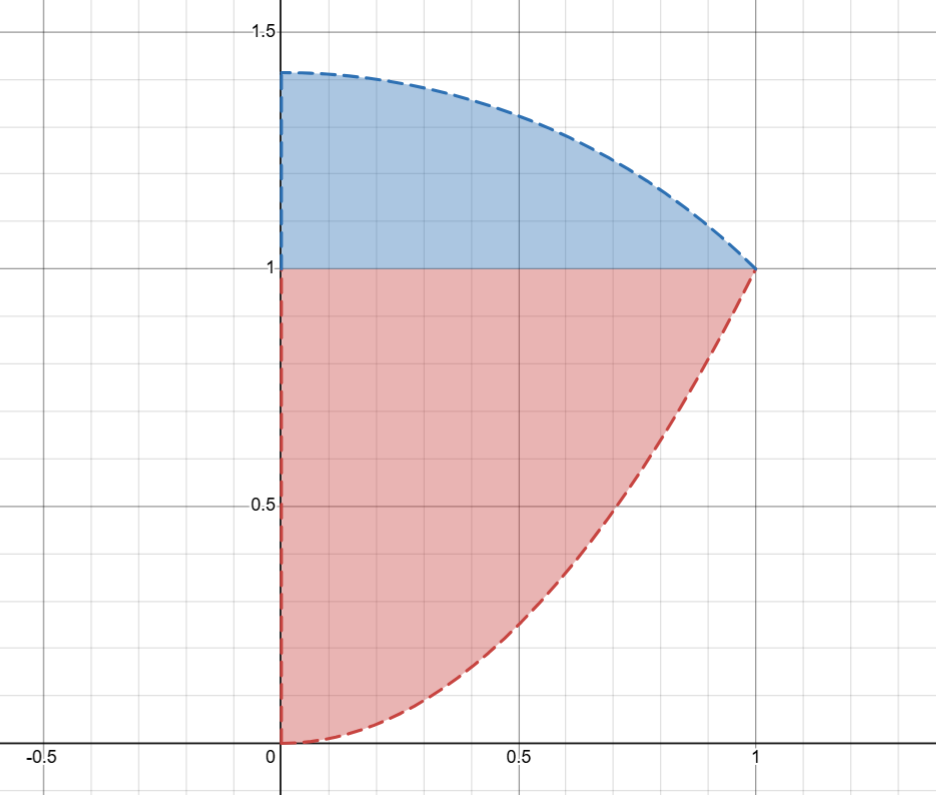
\includegraphics[width=0.3\linewidth]{Task1/Figure_shape.png}
    \caption{Задание 1. Область интегрирования.}
\end{figure}

Красным отмечена область левого интеграла, а синим - правого. Тогда можно записать двойной интеграл как
$$\int_{0}^{1}\, dy \int_{0}^{\sqrt{y}} f \, dx  + \int_{1}^{\sqrt{2}} \, dy\int_{0}^{\sqrt{2-y^2}} f \, dx = \iint\limits_D f dx\,dy $$

Где $D = \left\{0<x<\sqrt{y}\ \left\{0<y<1\right\}\right\} \cup \left\{0<x<\sqrt{2-y^{2}}\left\{1<y<\sqrt{2}\right\}\right\}$

Теперь попробуем поменять порядок интегрирования. Для этого нужно выразить $x$ через $y$ и наоборот.

Сначала выразим красную область. $x$ тут меняется внутри $(0,1)$, а $y$ найдем из неравенства.

$$0<x<\sqrt{y} \Rightarrow x^2 < y$$ 

И так как $x$ изначально был в $(0,1)$, то и $y$ будет идти до $1$. Тогда красная зона выражается так.

\begin{equation}
    x^2 < y < 1\left\{0 < x < 1\right\}
\end{equation}

Для синей области $x$ так же меняется внутри $(0,1)$. Этот $y$ тоже ограничен $1$, но уже снизу.

$$x<\sqrt{2-y^{2}} \Rightarrow x^2 < 2-y^2 \Rightarrow x^2-2 < -y^2 \Rightarrow y^2 < 2-x^2  \Rightarrow y < \sqrt{2-x^2}$$

\begin{equation}
    1 < y < \sqrt{2-x^2}\left\{0 < x < 1\right\}
\end{equation}

Теперь можно записывать это в виде интегралов, используя $(1)$ и $(2)$.

$$\int_{0}^{1}\, dy \int_{0}^{\sqrt{y}} f \, dx  + \int_{1}^{\sqrt{2}} \, dy\int_{0}^{\sqrt{2-y^2}} f \, dx = \int_{0}^{1}\, dx \int_{x^2}^{1} f \, dy  + \int_{0}^{1} \, dx\int_{1}^{\sqrt{2-x^2}} f \, dy $$

\href{https://www.desmos.com/Calculator/klqig4obxo}{Посмотреть задание в Desmos}
